
\documentclass[tikz,border=1.5pt]{standalone}
\usepackage{fontspec}
\usepackage{xeCJK}
\usepackage{amsmath,amssymb}
\usepackage{lmodern}
\setmainfont{Arial}
\setsansfont{Arial}
\setCJKmainfont{Microsoft YaHei}
\renewcommand{\familydefault}{\sfdefault}
\usetikzlibrary{arrows.meta,calc}
\definecolor{Blue}{HTML}{1479E0}
\definecolor{Orange}{HTML}{F28E2B}
\definecolor{Green}{HTML}{159B75}
\definecolor{Ink}{HTML}{202D3D}
\definecolor{Neutral}{HTML}{65758A}
\definecolor{Line}{HTML}{C6D0DB}
\tikzset{
  every node/.style={font=\fontsize{8.6}{10.2}\selectfont,text=black,inner sep=0pt,outer sep=0pt},
  arr/.style={-{Stealth[length=4.5pt,width=3.5pt]},line width=.8pt,draw=Ink},
  bluearr/.style={arr,draw=Blue},
  orangearr/.style={arr,draw=Orange},
  greenarr/.style={arr,draw=Green},
  histarr/.style={arr,draw=Neutral,dash pattern=on 3pt off 2pt},
}
\begin{document}
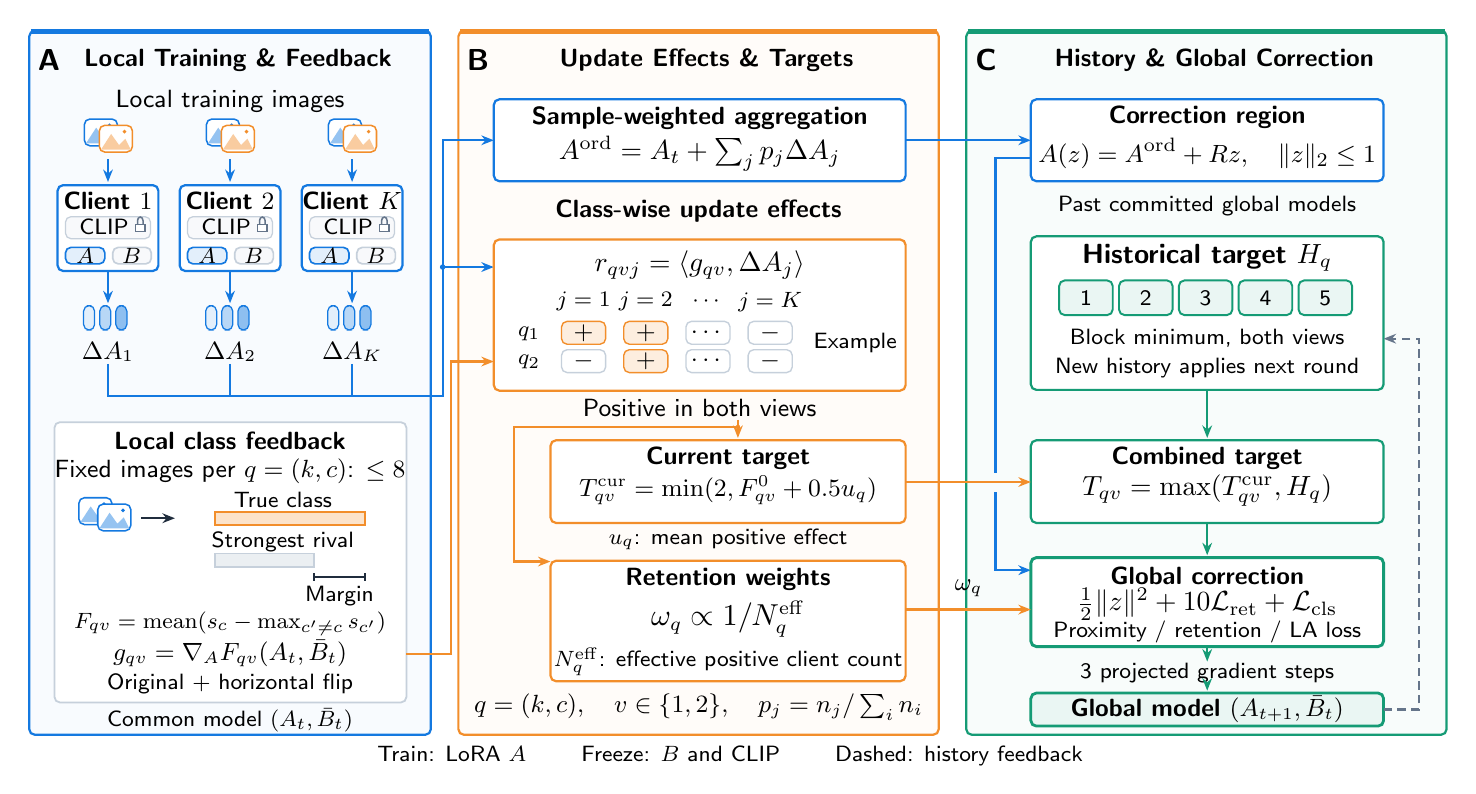
\begin{tikzpicture}[x=1cm,y=-1cm]
\path[use as bounding box] (-.02,-.02) rectangle (18.02,9.35);

\draw[draw=Blue,fill=Blue!3,rounded corners=2pt,line width=0.8pt] (0,0.02) rectangle (5.1,8.96);
\draw[draw=Blue,line width=2pt] (0.02,.03) -- (5.08,.03);
\node[font=\fontsize{10.5}{12.2}\selectfont\bfseries] (label0) at (0.25,0.39) {A};
\path let \p1=(label0.south west), \p2=(label0.north east) in \pgfextra{\typeout{NODEBOUNDS|label0|\x1|\y1|\x2|\y2}};
\node[font=\fontsize{9.3}{11.0}\selectfont\bfseries] (label1) at (2.65,0.39) {Local Training \& Feedback};
\path let \p1=(label1.south west), \p2=(label1.north east) in \pgfextra{\typeout{NODEBOUNDS|label1|\x1|\y1|\x2|\y2}};
\draw[draw=Orange,fill=Orange!3,rounded corners=2pt,line width=0.8pt] (5.45,0.02) rectangle (11.55,8.96);
\draw[draw=Orange,line width=2pt] (5.47,.03) -- (11.530000000000001,.03);
\node[font=\fontsize{10.5}{12.2}\selectfont\bfseries] (label2) at (5.7,0.39) {B};
\path let \p1=(label2.south west), \p2=(label2.north east) in \pgfextra{\typeout{NODEBOUNDS|label2|\x1|\y1|\x2|\y2}};
\node[font=\fontsize{9.3}{11.0}\selectfont\bfseries] (label3) at (8.6,0.39) {Update Effects \& Targets};
\path let \p1=(label3.south west), \p2=(label3.north east) in \pgfextra{\typeout{NODEBOUNDS|label3|\x1|\y1|\x2|\y2}};
\draw[draw=Green,fill=Green!3,rounded corners=2pt,line width=0.8pt] (11.9,0.02) rectangle (18,8.96);
\draw[draw=Green,line width=2pt] (11.92,.03) -- (17.98,.03);
\node[font=\fontsize{10.5}{12.2}\selectfont\bfseries] (label4) at (12.15,0.39) {C};
\path let \p1=(label4.south west), \p2=(label4.north east) in \pgfextra{\typeout{NODEBOUNDS|label4|\x1|\y1|\x2|\y2}};
\node[font=\fontsize{9.3}{11.0}\selectfont\bfseries] (label5) at (15.049999999999999,0.39) {History \& Global Correction};
\path let \p1=(label5.south west), \p2=(label5.north east) in \pgfextra{\typeout{NODEBOUNDS|label5|\x1|\y1|\x2|\y2}};
\node[font=\fontsize{8.6}{10.299999999999999}\selectfont] (label6) at (2.55,0.92) {Local training images};
\path let \p1=(label6.south west), \p2=(label6.north east) in \pgfextra{\typeout{NODEBOUNDS|label6|\x1|\y1|\x2|\y2}};
\draw[draw=Blue,fill=white,rounded corners=2pt,line width=0.55pt] (0.7,1.14) rectangle (1.1199999999999999,1.48);
\fill[Blue!45] (0.72,1.45) -- (0.85,1.25) -- (0.95,1.39) -- (1.03,1.3099999999999998) -- (1.1,1.45) -- cycle;
\fill[Blue] (1.02,1.22) circle (.025);
\draw[draw=Orange,fill=white,rounded corners=2pt,line width=0.55pt] (0.89,1.22) rectangle (1.31,1.56);
\fill[Orange!45] (0.91,1.53) -- (1.04,1.33) -- (1.1400000000000001,1.47) -- (1.22,1.39) -- (1.29,1.53) -- cycle;
\fill[Orange] (1.21,1.3) circle (.025);
\draw[bluearr] (1.0,1.65) -- (1.0,1.94);
\draw[draw=Blue,fill=white,rounded corners=2pt,line width=0.8pt] (0.36,1.98) rectangle (1.6400000000000001,3.07);
\node[font=\fontsize{8.8}{10.5}\selectfont\bfseries] (label7) at (1.0,2.18) {Client $1$};
\path let \p1=(label7.south west), \p2=(label7.north east) in \pgfextra{\typeout{NODEBOUNDS|label7|\x1|\y1|\x2|\y2}};
\draw[draw=Line,fill=Line!12,rounded corners=2pt,line width=0.45pt] (0.45999999999999996,2.38) rectangle (1.54,2.66);
\node[font=\fontsize{8.3}{10.0}\selectfont] (label8) at (0.95,2.51) {CLIP};
\path let \p1=(label8.south west), \p2=(label8.north east) in \pgfextra{\typeout{NODEBOUNDS|label8|\x1|\y1|\x2|\y2}};
\draw[draw=Neutral,line width=.55pt] (1.375,2.48) -- (1.375,2.43) arc[start angle=180,end angle=0,x radius=.035cm,y radius=.045cm] -- (1.4449999999999998,2.48);
\draw[draw=Neutral,fill=white,line width=.55pt] (1.3499999999999999,2.48) rectangle (1.47,2.57);
\draw[draw=Blue,fill=Blue!12,rounded corners=2pt,line width=0.6pt] (0.45999999999999996,2.77) rectangle (0.96,2.98);
\draw[draw=Line,fill=Line!12,rounded corners=2pt,line width=0.6pt] (1.06,2.77) rectangle (1.55,2.98);
\node[font=\fontsize{8.5}{10.2}\selectfont\bfseries] (label9) at (0.71,2.875) {$A$};
\path let \p1=(label9.south west), \p2=(label9.north east) in \pgfextra{\typeout{NODEBOUNDS|label9|\x1|\y1|\x2|\y2}};
\node[font=\fontsize{8.5}{10.2}\selectfont] (label10) at (1.3,2.875) {$B$};
\path let \p1=(label10.south west), \p2=(label10.north east) in \pgfextra{\typeout{NODEBOUNDS|label10|\x1|\y1|\x2|\y2}};
\draw[bluearr] (1.0,3.08) -- (1.0,3.48);
\draw[draw=Blue,fill=Blue!12,rounded corners=2pt,line width=0.45pt] (0.69,3.51) rectangle (0.83,3.82);
\draw[draw=Blue,fill=Blue!30,rounded corners=2pt,line width=0.45pt] (0.8949999999999999,3.51) rectangle (1.035,3.82);
\draw[draw=Blue,fill=Blue!48,rounded corners=2pt,line width=0.45pt] (1.0999999999999999,3.51) rectangle (1.24,3.82);
\node[font=\fontsize{9.2}{10.899999999999999}\selectfont] (label11) at (1.0,4.1) {$\Delta A_{1}$};
\path let \p1=(label11.south west), \p2=(label11.north east) in \pgfextra{\typeout{NODEBOUNDS|label11|\x1|\y1|\x2|\y2}};
\draw[draw=Blue,fill=white,rounded corners=2pt,line width=0.55pt] (2.25,1.14) rectangle (2.67,1.48);
\fill[Blue!45] (2.27,1.45) -- (2.4,1.25) -- (2.5,1.39) -- (2.58,1.3099999999999998) -- (2.65,1.45) -- cycle;
\fill[Blue] (2.57,1.22) circle (.025);
\draw[draw=Orange,fill=white,rounded corners=2pt,line width=0.55pt] (2.44,1.22) rectangle (2.86,1.56);
\fill[Orange!45] (2.46,1.53) -- (2.59,1.33) -- (2.69,1.47) -- (2.77,1.39) -- (2.84,1.53) -- cycle;
\fill[Orange] (2.76,1.3) circle (.025);
\draw[bluearr] (2.55,1.65) -- (2.55,1.94);
\draw[draw=Blue,fill=white,rounded corners=2pt,line width=0.8pt] (1.9099999999999997,1.98) rectangle (3.19,3.07);
\node[font=\fontsize{8.8}{10.5}\selectfont\bfseries] (label12) at (2.55,2.18) {Client $2$};
\path let \p1=(label12.south west), \p2=(label12.north east) in \pgfextra{\typeout{NODEBOUNDS|label12|\x1|\y1|\x2|\y2}};
\draw[draw=Line,fill=Line!12,rounded corners=2pt,line width=0.45pt] (2.01,2.38) rectangle (3.09,2.66);
\node[font=\fontsize{8.3}{10.0}\selectfont] (label13) at (2.5,2.51) {CLIP};
\path let \p1=(label13.south west), \p2=(label13.north east) in \pgfextra{\typeout{NODEBOUNDS|label13|\x1|\y1|\x2|\y2}};
\draw[draw=Neutral,line width=.55pt] (2.925,2.48) -- (2.925,2.43) arc[start angle=180,end angle=0,x radius=.035cm,y radius=.045cm] -- (2.995,2.48);
\draw[draw=Neutral,fill=white,line width=.55pt] (2.9,2.48) rectangle (3.02,2.57);
\draw[draw=Blue,fill=Blue!12,rounded corners=2pt,line width=0.6pt] (2.01,2.77) rectangle (2.51,2.98);
\draw[draw=Line,fill=Line!12,rounded corners=2pt,line width=0.6pt] (2.61,2.77) rectangle (3.0999999999999996,2.98);
\node[font=\fontsize{8.5}{10.2}\selectfont\bfseries] (label14) at (2.26,2.875) {$A$};
\path let \p1=(label14.south west), \p2=(label14.north east) in \pgfextra{\typeout{NODEBOUNDS|label14|\x1|\y1|\x2|\y2}};
\node[font=\fontsize{8.5}{10.2}\selectfont] (label15) at (2.8499999999999996,2.875) {$B$};
\path let \p1=(label15.south west), \p2=(label15.north east) in \pgfextra{\typeout{NODEBOUNDS|label15|\x1|\y1|\x2|\y2}};
\draw[bluearr] (2.55,3.08) -- (2.55,3.48);
\draw[draw=Blue,fill=Blue!12,rounded corners=2pt,line width=0.45pt] (2.2399999999999998,3.51) rectangle (2.38,3.82);
\draw[draw=Blue,fill=Blue!30,rounded corners=2pt,line width=0.45pt] (2.445,3.51) rectangle (2.585,3.82);
\draw[draw=Blue,fill=Blue!48,rounded corners=2pt,line width=0.45pt] (2.65,3.51) rectangle (2.79,3.82);
\node[font=\fontsize{9.2}{10.899999999999999}\selectfont] (label16) at (2.55,4.1) {$\Delta A_{2}$};
\path let \p1=(label16.south west), \p2=(label16.north east) in \pgfextra{\typeout{NODEBOUNDS|label16|\x1|\y1|\x2|\y2}};
\draw[draw=Blue,fill=white,rounded corners=2pt,line width=0.55pt] (3.8,1.14) rectangle (4.22,1.48);
\fill[Blue!45] (3.82,1.45) -- (3.9499999999999997,1.25) -- (4.05,1.39) -- (4.13,1.3099999999999998) -- (4.2,1.45) -- cycle;
\fill[Blue] (4.12,1.22) circle (.025);
\draw[draw=Orange,fill=white,rounded corners=2pt,line width=0.55pt] (3.9899999999999998,1.22) rectangle (4.41,1.56);
\fill[Orange!45] (4.01,1.53) -- (4.14,1.33) -- (4.24,1.47) -- (4.319999999999999,1.39) -- (4.39,1.53) -- cycle;
\fill[Orange] (4.31,1.3) circle (.025);
\draw[bluearr] (4.1,1.65) -- (4.1,1.94);
\draw[draw=Blue,fill=white,rounded corners=2pt,line width=0.8pt] (3.4599999999999995,1.98) rectangle (4.739999999999999,3.07);
\node[font=\fontsize{8.8}{10.5}\selectfont\bfseries] (label17) at (4.1,2.18) {Client $K$};
\path let \p1=(label17.south west), \p2=(label17.north east) in \pgfextra{\typeout{NODEBOUNDS|label17|\x1|\y1|\x2|\y2}};
\draw[draw=Line,fill=Line!12,rounded corners=2pt,line width=0.45pt] (3.5599999999999996,2.38) rectangle (4.64,2.66);
\node[font=\fontsize{8.3}{10.0}\selectfont] (label18) at (4.05,2.51) {CLIP};
\path let \p1=(label18.south west), \p2=(label18.north east) in \pgfextra{\typeout{NODEBOUNDS|label18|\x1|\y1|\x2|\y2}};
\draw[draw=Neutral,line width=.55pt] (4.475,2.48) -- (4.475,2.43) arc[start angle=180,end angle=0,x radius=.035cm,y radius=.045cm] -- (4.545,2.48);
\draw[draw=Neutral,fill=white,line width=.55pt] (4.45,2.48) rectangle (4.569999999999999,2.57);
\draw[draw=Blue,fill=Blue!12,rounded corners=2pt,line width=0.6pt] (3.5599999999999996,2.77) rectangle (4.06,2.98);
\draw[draw=Line,fill=Line!12,rounded corners=2pt,line width=0.6pt] (4.159999999999999,2.77) rectangle (4.6499999999999995,2.98);
\node[font=\fontsize{8.5}{10.2}\selectfont\bfseries] (label19) at (3.8099999999999996,2.875) {$A$};
\path let \p1=(label19.south west), \p2=(label19.north east) in \pgfextra{\typeout{NODEBOUNDS|label19|\x1|\y1|\x2|\y2}};
\node[font=\fontsize{8.5}{10.2}\selectfont] (label20) at (4.3999999999999995,2.875) {$B$};
\path let \p1=(label20.south west), \p2=(label20.north east) in \pgfextra{\typeout{NODEBOUNDS|label20|\x1|\y1|\x2|\y2}};
\draw[bluearr] (4.1,3.08) -- (4.1,3.48);
\draw[draw=Blue,fill=Blue!12,rounded corners=2pt,line width=0.45pt] (3.7899999999999996,3.51) rectangle (3.9299999999999997,3.82);
\draw[draw=Blue,fill=Blue!30,rounded corners=2pt,line width=0.45pt] (3.9949999999999997,3.51) rectangle (4.135,3.82);
\draw[draw=Blue,fill=Blue!48,rounded corners=2pt,line width=0.45pt] (4.199999999999999,3.51) rectangle (4.34,3.82);
\node[font=\fontsize{9.2}{10.899999999999999}\selectfont] (label21) at (4.1,4.1) {$\Delta A_{K}$};
\path let \p1=(label21.south west), \p2=(label21.north east) in \pgfextra{\typeout{NODEBOUNDS|label21|\x1|\y1|\x2|\y2}};
\draw[draw=Blue,line width=.7pt] (1,4.25) -- (1,4.66) -- (4.8,4.66);
\draw[draw=Blue,line width=.7pt] (2.55,4.25) -- (2.55,4.66);
\draw[draw=Blue,line width=.7pt] (4.1,4.25) -- (4.1,4.66);
\draw[bluearr] (4.8,4.66) -- (5.25,4.66) -- (5.25,1.41) -- (5.9,1.41);
\draw[bluearr] (5.25,3.02) -- (5.9,3.02);
\fill[Blue] (5.25,3.02) circle (.035);
\draw[draw=Line,fill=white,rounded corners=2pt,line width=0.65pt] (0.32,4.99) rectangle (4.79,8.55);
\node[font=\fontsize{9.4}{11.1}\selectfont\bfseries] (label22) at (2.55,5.23) {Local class feedback};
\path let \p1=(label22.south west), \p2=(label22.north east) in \pgfextra{\typeout{NODEBOUNDS|label22|\x1|\y1|\x2|\y2}};
\node[font=\fontsize{8.6}{10.299999999999999}\selectfont] (label23) at (2.55,5.61) {Fixed images per $q=(k,c)$: $\leq8$};
\path let \p1=(label23.south west), \p2=(label23.north east) in \pgfextra{\typeout{NODEBOUNDS|label23|\x1|\y1|\x2|\y2}};
\draw[draw=Blue,fill=white,rounded corners=2pt,line width=0.55pt] (0.63,5.95) rectangle (1.05,6.29);
\fill[Blue!45] (0.65,6.26) -- (0.78,6.0600000000000005) -- (0.88,6.2) -- (0.96,6.12) -- (1.03,6.26) -- cycle;
\fill[Blue] (0.95,6.03) circle (.025);
\draw[draw=Blue,fill=white,rounded corners=2pt,line width=0.55pt] (0.87,6.03) rectangle (1.29,6.37);
\fill[Blue!45] (0.89,6.34) -- (1.02,6.140000000000001) -- (1.12,6.28) -- (1.2,6.2) -- (1.27,6.34) -- cycle;
\fill[Blue] (1.19,6.11) circle (.025);
\draw[arr] (1.42,6.21) -- (1.85,6.21);
\node[font=\fontsize{8.3}{10.0}\selectfont] (label24) at (3.22,5.98) {True class};
\path let \p1=(label24.south west), \p2=(label24.north east) in \pgfextra{\typeout{NODEBOUNDS|label24|\x1|\y1|\x2|\y2}};
\node[font=\fontsize{8.3}{10.0}\selectfont] (label25) at (3.22,6.51) {Strongest rival};
\path let \p1=(label25.south west), \p2=(label25.north east) in \pgfextra{\typeout{NODEBOUNDS|label25|\x1|\y1|\x2|\y2}};
\draw[draw=Orange,fill=Orange!25,line width=.6pt] (2.36,6.13) rectangle (4.26,6.30);
\draw[draw=Line,fill=Line!35,line width=.6pt] (2.36,6.66) rectangle (3.62,6.83);
\draw[draw=Ink,line width=.6pt] (3.62,6.96) -- (4.26,6.96);
\draw[draw=Ink,line width=.6pt] (3.62,6.91) -- (3.62,7.01) (4.26,6.91) -- (4.26,7.01);
\node[font=\fontsize{8.3}{10.0}\selectfont] (label26) at (3.94,7.2) {Margin};
\path let \p1=(label26.south west), \p2=(label26.north east) in \pgfextra{\typeout{NODEBOUNDS|label26|\x1|\y1|\x2|\y2}};
\node[font=\fontsize{8.5}{10.2}\selectfont] (label27) at (2.55,7.55) {$F_{qv}=\operatorname{mean}(s_c-\max_{c'\ne c}s_{c'})$};
\path let \p1=(label27.south west), \p2=(label27.north east) in \pgfextra{\typeout{NODEBOUNDS|label27|\x1|\y1|\x2|\y2}};
\node[font=\fontsize{9.0}{10.7}\selectfont] (label28) at (2.55,7.93) {$g_{qv}=\nabla_A F_{qv}(A_t,\bar B_t)$};
\path let \p1=(label28.south west), \p2=(label28.north east) in \pgfextra{\typeout{NODEBOUNDS|label28|\x1|\y1|\x2|\y2}};
\node[font=\fontsize{8.3}{10.0}\selectfont] (label29) at (2.55,8.32) {Original + horizontal flip};
\path let \p1=(label29.south west), \p2=(label29.north east) in \pgfextra{\typeout{NODEBOUNDS|label29|\x1|\y1|\x2|\y2}};
\draw[orangearr] (4.79,7.93) -- (5.36,7.93) -- (5.36,4.22) -- (5.9,4.22);
\draw[draw=Blue,fill=white,rounded corners=2pt,line width=0.8pt] (5.9,0.89) rectangle (11.13,1.93);
\node[font=\fontsize{9.3}{11.0}\selectfont\bfseries] (label30) at (8.515,1.13) {Sample-weighted aggregation};
\path let \p1=(label30.south west), \p2=(label30.north east) in \pgfextra{\typeout{NODEBOUNDS|label30|\x1|\y1|\x2|\y2}};
\node[font=\fontsize{10}{11.7}\selectfont] (label31) at (8.515,1.58) {$A^{\mathrm{ord}}=A_t+\sum_j p_j\Delta A_j$};
\path let \p1=(label31.south west), \p2=(label31.north east) in \pgfextra{\typeout{NODEBOUNDS|label31|\x1|\y1|\x2|\y2}};
\draw[bluearr] (11.13,1.41) -- (12.72,1.41);
\node[font=\fontsize{9.2}{10.899999999999999}\selectfont\bfseries] (label32) at (8.5,2.31) {Class-wise update effects};
\path let \p1=(label32.south west), \p2=(label32.north east) in \pgfextra{\typeout{NODEBOUNDS|label32|\x1|\y1|\x2|\y2}};
\draw[draw=Orange,fill=white,rounded corners=2pt,line width=0.8pt] (5.9,2.67) rectangle (11.13,4.59);
\node[font=\fontsize{10}{11.7}\selectfont] (label33) at (8.515,2.99) {$r_{qvj}=\langle g_{qv},\Delta A_j\rangle$};
\path let \p1=(label33.south west), \p2=(label33.north east) in \pgfextra{\typeout{NODEBOUNDS|label33|\x1|\y1|\x2|\y2}};
\node[font=\fontsize{8.3}{10.0}\selectfont] (label34) at (7.04,3.46) {$j=1$};
\path let \p1=(label34.south west), \p2=(label34.north east) in \pgfextra{\typeout{NODEBOUNDS|label34|\x1|\y1|\x2|\y2}};
\node[font=\fontsize{8.3}{10.0}\selectfont] (label35) at (7.83,3.46) {$j=2$};
\path let \p1=(label35.south west), \p2=(label35.north east) in \pgfextra{\typeout{NODEBOUNDS|label35|\x1|\y1|\x2|\y2}};
\node[font=\fontsize{8.3}{10.0}\selectfont] (label36) at (8.620000000000001,3.46) {$\cdots$};
\path let \p1=(label36.south west), \p2=(label36.north east) in \pgfextra{\typeout{NODEBOUNDS|label36|\x1|\y1|\x2|\y2}};
\node[font=\fontsize{8.3}{10.0}\selectfont] (label37) at (9.41,3.46) {$j=K$};
\path let \p1=(label37.south west), \p2=(label37.north east) in \pgfextra{\typeout{NODEBOUNDS|label37|\x1|\y1|\x2|\y2}};
\node[font=\fontsize{8.5}{10.2}\selectfont] (label38) at (6.35,3.87) {$q_1$};
\path let \p1=(label38.south west), \p2=(label38.north east) in \pgfextra{\typeout{NODEBOUNDS|label38|\x1|\y1|\x2|\y2}};
\draw[draw=Orange,fill=Orange!15,rounded corners=2pt,line width=0.5pt] (6.76,3.71) rectangle (7.32,4.0);
\node[font=\fontsize{9}{10.7}\selectfont] (label39) at (7.04,3.855) {+};
\path let \p1=(label39.south west), \p2=(label39.north east) in \pgfextra{\typeout{NODEBOUNDS|label39|\x1|\y1|\x2|\y2}};
\draw[draw=Orange,fill=Orange!15,rounded corners=2pt,line width=0.5pt] (7.55,3.71) rectangle (8.11,4.0);
\node[font=\fontsize{9}{10.7}\selectfont] (label40) at (7.83,3.855) {+};
\path let \p1=(label40.south west), \p2=(label40.north east) in \pgfextra{\typeout{NODEBOUNDS|label40|\x1|\y1|\x2|\y2}};
\draw[draw=Line,fill=white,rounded corners=2pt,line width=0.5pt] (8.34,3.71) rectangle (8.9,4.0);
\node[font=\fontsize{9}{10.7}\selectfont] (label41) at (8.620000000000001,3.855) {$\cdots$};
\path let \p1=(label41.south west), \p2=(label41.north east) in \pgfextra{\typeout{NODEBOUNDS|label41|\x1|\y1|\x2|\y2}};
\draw[draw=Line,fill=white,rounded corners=2pt,line width=0.5pt] (9.129999999999999,3.71) rectangle (9.690000000000001,4.0);
\node[font=\fontsize{9}{10.7}\selectfont] (label42) at (9.41,3.855) {$-$};
\path let \p1=(label42.south west), \p2=(label42.north east) in \pgfextra{\typeout{NODEBOUNDS|label42|\x1|\y1|\x2|\y2}};
\node[font=\fontsize{8.5}{10.2}\selectfont] (label43) at (6.35,4.23) {$q_2$};
\path let \p1=(label43.south west), \p2=(label43.north east) in \pgfextra{\typeout{NODEBOUNDS|label43|\x1|\y1|\x2|\y2}};
\draw[draw=Line,fill=white,rounded corners=2pt,line width=0.5pt] (6.76,4.07) rectangle (7.32,4.36);
\node[font=\fontsize{9}{10.7}\selectfont] (label44) at (7.04,4.215) {$-$};
\path let \p1=(label44.south west), \p2=(label44.north east) in \pgfextra{\typeout{NODEBOUNDS|label44|\x1|\y1|\x2|\y2}};
\draw[draw=Orange,fill=Orange!15,rounded corners=2pt,line width=0.5pt] (7.55,4.07) rectangle (8.11,4.36);
\node[font=\fontsize{9}{10.7}\selectfont] (label45) at (7.83,4.215) {+};
\path let \p1=(label45.south west), \p2=(label45.north east) in \pgfextra{\typeout{NODEBOUNDS|label45|\x1|\y1|\x2|\y2}};
\draw[draw=Line,fill=white,rounded corners=2pt,line width=0.5pt] (8.34,4.07) rectangle (8.9,4.36);
\node[font=\fontsize{9}{10.7}\selectfont] (label46) at (8.620000000000001,4.215) {$\cdots$};
\path let \p1=(label46.south west), \p2=(label46.north east) in \pgfextra{\typeout{NODEBOUNDS|label46|\x1|\y1|\x2|\y2}};
\draw[draw=Line,fill=white,rounded corners=2pt,line width=0.5pt] (9.129999999999999,4.07) rectangle (9.690000000000001,4.36);
\node[font=\fontsize{9}{10.7}\selectfont] (label47) at (9.41,4.215) {$-$};
\path let \p1=(label47.south west), \p2=(label47.north east) in \pgfextra{\typeout{NODEBOUNDS|label47|\x1|\y1|\x2|\y2}};
\node[font=\fontsize{8.3}{10.0}\selectfont] (label48) at (10.49,3.99) {Example};
\path let \p1=(label48.south west), \p2=(label48.north east) in \pgfextra{\typeout{NODEBOUNDS|label48|\x1|\y1|\x2|\y2}};
\node[font=\fontsize{8.6}{10.299999999999999}\selectfont] (label49) at (8.515,4.81) {Positive in both views};
\path let \p1=(label49.south west), \p2=(label49.north east) in \pgfextra{\typeout{NODEBOUNDS|label49|\x1|\y1|\x2|\y2}};
\draw[orangearr] (9.0,4.96) -- (9.0,5.19);
\draw[draw=Orange,fill=white,rounded corners=2pt,line width=0.8pt] (6.62,5.22) rectangle (11.13,6.27);
\node[font=\fontsize{9.0}{10.7}\selectfont\bfseries] (label50) at (8.875,5.45) {Current target};
\path let \p1=(label50.south west), \p2=(label50.north east) in \pgfextra{\typeout{NODEBOUNDS|label50|\x1|\y1|\x2|\y2}};
\node[font=\fontsize{9.1}{10.799999999999999}\selectfont] (label51) at (8.875,5.85) {$T^{\mathrm{cur}}_{qv}=\min(2,F^0_{qv}+0.5u_q)$};
\path let \p1=(label51.south west), \p2=(label51.north east) in \pgfextra{\typeout{NODEBOUNDS|label51|\x1|\y1|\x2|\y2}};
\node[font=\fontsize{8.4}{10.1}\selectfont] (label52) at (8.875,6.48) {$u_q$: mean positive effect};
\path let \p1=(label52.south west), \p2=(label52.north east) in \pgfextra{\typeout{NODEBOUNDS|label52|\x1|\y1|\x2|\y2}};
\draw[orangearr] (9.0,5.05) -- (6.16,5.05) -- (6.16,6.76) -- (6.62,6.76);
\fill[Orange] (9.0,5.05) circle (.028);
\draw[draw=Orange,fill=white,rounded corners=2pt,line width=0.8pt] (6.62,6.75) rectangle (11.13,8.28);
\node[font=\fontsize{9.0}{10.7}\selectfont\bfseries] (label53) at (8.875,6.99) {Retention weights};
\path let \p1=(label53.south west), \p2=(label53.north east) in \pgfextra{\typeout{NODEBOUNDS|label53|\x1|\y1|\x2|\y2}};
\node[font=\fontsize{10.5}{12.2}\selectfont] (label54) at (8.875,7.49) {$\omega_q\propto 1/N_q^{\mathrm{eff}}$};
\path let \p1=(label54.south west), \p2=(label54.north east) in \pgfextra{\typeout{NODEBOUNDS|label54|\x1|\y1|\x2|\y2}};
\node[font=\fontsize{8.3}{10.0}\selectfont] (label55) at (8.875,8.03) {$N_q^{\mathrm{eff}}$: effective positive client count};
\path let \p1=(label55.south west), \p2=(label55.north east) in \pgfextra{\typeout{NODEBOUNDS|label55|\x1|\y1|\x2|\y2}};
\node[font=\fontsize{8.7}{10.399999999999999}\selectfont] (label56) at (8.5,8.61) {$q=(k,c),\quad v\in\{1,2\},\quad p_j=n_j/\sum_i n_i$};
\path let \p1=(label56.south west), \p2=(label56.north east) in \pgfextra{\typeout{NODEBOUNDS|label56|\x1|\y1|\x2|\y2}};
\draw[draw=Blue,fill=white,rounded corners=2pt,line width=0.8pt] (12.72,0.89) rectangle (17.2,1.93);
\node[font=\fontsize{9.3}{11.0}\selectfont\bfseries] (label57) at (14.96,1.12) {Correction region};
\path let \p1=(label57.south west), \p2=(label57.north east) in \pgfextra{\typeout{NODEBOUNDS|label57|\x1|\y1|\x2|\y2}};
\node[font=\fontsize{9.4}{11.1}\selectfont] (label58) at (14.96,1.58) {$A(z)=A^{\mathrm{ord}}+Rz,\quad \|z\|_2\leq1$};
\path let \p1=(label58.south west), \p2=(label58.north east) in \pgfextra{\typeout{NODEBOUNDS|label58|\x1|\y1|\x2|\y2}};
\draw[draw=Blue,line width=.8pt] (12.72,1.64) -- (12.27,1.64) -- (12.27,5.63);
\draw[bluearr] (12.27,5.88) -- (12.27,6.87) -- (12.72,6.87);
\draw[draw=Green,fill=white,rounded corners=2pt,line width=0.8pt] (12.72,2.63) rectangle (17.2,4.58);
\node[font=\fontsize{9.6}{11.299999999999999}\selectfont\bfseries] (label59) at (14.96,2.9) {Historical target $H_q$};
\path let \p1=(label59.south west), \p2=(label59.north east) in \pgfextra{\typeout{NODEBOUNDS|label59|\x1|\y1|\x2|\y2}};
\draw[draw=Green,fill=Green!9,rounded corners=2pt,line width=0.7pt] (13.08,3.19) rectangle (13.76,3.63);
\node[font=\fontsize{8.5}{10.2}\selectfont] (label60) at (13.42,3.41) {1};
\path let \p1=(label60.south west), \p2=(label60.north east) in \pgfextra{\typeout{NODEBOUNDS|label60|\x1|\y1|\x2|\y2}};
\draw[draw=Green,fill=Green!9,rounded corners=2pt,line width=0.7pt] (13.84,3.19) rectangle (14.52,3.63);
\node[font=\fontsize{8.5}{10.2}\selectfont] (label61) at (14.18,3.41) {2};
\path let \p1=(label61.south west), \p2=(label61.north east) in \pgfextra{\typeout{NODEBOUNDS|label61|\x1|\y1|\x2|\y2}};
\draw[draw=Green,fill=Green!9,rounded corners=2pt,line width=0.7pt] (14.6,3.19) rectangle (15.28,3.63);
\node[font=\fontsize{8.5}{10.2}\selectfont] (label62) at (14.94,3.41) {3};
\path let \p1=(label62.south west), \p2=(label62.north east) in \pgfextra{\typeout{NODEBOUNDS|label62|\x1|\y1|\x2|\y2}};
\draw[draw=Green,fill=Green!9,rounded corners=2pt,line width=0.7pt] (15.36,3.19) rectangle (16.04,3.63);
\node[font=\fontsize{8.5}{10.2}\selectfont] (label63) at (15.7,3.41) {4};
\path let \p1=(label63.south west), \p2=(label63.north east) in \pgfextra{\typeout{NODEBOUNDS|label63|\x1|\y1|\x2|\y2}};
\draw[draw=Green,fill=Green!9,rounded corners=2pt,line width=0.7pt] (16.12,3.19) rectangle (16.8,3.63);
\node[font=\fontsize{8.5}{10.2}\selectfont] (label64) at (16.46,3.41) {5};
\path let \p1=(label64.south west), \p2=(label64.north east) in \pgfextra{\typeout{NODEBOUNDS|label64|\x1|\y1|\x2|\y2}};
\node[font=\fontsize{8.4}{10.1}\selectfont] (label65) at (14.96,3.92) {Block minimum, both views};
\path let \p1=(label65.south west), \p2=(label65.north east) in \pgfextra{\typeout{NODEBOUNDS|label65|\x1|\y1|\x2|\y2}};
\node[font=\fontsize{8.3}{10.0}\selectfont] (label66) at (14.96,4.3) {New history applies next round};
\path let \p1=(label66.south west), \p2=(label66.north east) in \pgfextra{\typeout{NODEBOUNDS|label66|\x1|\y1|\x2|\y2}};
\draw[greenarr] (14.96,4.58) -- (14.96,5.19);
\draw[draw=Green,fill=white,rounded corners=2pt,line width=0.8pt] (12.72,5.22) rectangle (17.2,6.27);
\node[font=\fontsize{8.7}{10.399999999999999}\selectfont\bfseries] (label67) at (14.96,5.45) {Combined target};
\path let \p1=(label67.south west), \p2=(label67.north east) in \pgfextra{\typeout{NODEBOUNDS|label67|\x1|\y1|\x2|\y2}};
\node[font=\fontsize{10}{11.7}\selectfont] (label68) at (14.96,5.86) {$T_{qv}=\max(T^{\mathrm{cur}}_{qv},H_q)$};
\path let \p1=(label68.south west), \p2=(label68.north east) in \pgfextra{\typeout{NODEBOUNDS|label68|\x1|\y1|\x2|\y2}};
\draw[orangearr] (11.13,5.75) -- (12.72,5.75);
\draw[greenarr] (14.96,6.27) -- (14.96,6.68);
\draw[draw=Green,fill=white,rounded corners=2pt,line width=1.05pt] (12.72,6.71) rectangle (17.2,7.84);
\node[font=\fontsize{9.3}{11.0}\selectfont\bfseries] (label69) at (14.96,6.94) {Global correction};
\path let \p1=(label69.south west), \p2=(label69.north east) in \pgfextra{\typeout{NODEBOUNDS|label69|\x1|\y1|\x2|\y2}};
\node[font=\fontsize{10.0}{11.7}\selectfont] (label70) at (14.96,7.3) {$\frac12\|z\|^2+10\mathcal L_{\rm ret}+\mathcal L_{\rm cls}$};
\path let \p1=(label70.south west), \p2=(label70.north east) in \pgfextra{\typeout{NODEBOUNDS|label70|\x1|\y1|\x2|\y2}};
\node[font=\fontsize{8.3}{10.0}\selectfont] (label71) at (14.96,7.65) {Proximity / retention / LA loss};
\path let \p1=(label71.south west), \p2=(label71.north east) in \pgfextra{\typeout{NODEBOUNDS|label71|\x1|\y1|\x2|\y2}};
\draw[orangearr] (11.13,7.37) -- (12.72,7.37);
\node[font=\fontsize{9}{10.7}\selectfont] (label72) at (11.93,7.1) {$\omega_q$};
\path let \p1=(label72.south west), \p2=(label72.north east) in \pgfextra{\typeout{NODEBOUNDS|label72|\x1|\y1|\x2|\y2}};
\draw[greenarr] (14.96,7.84) -- (14.96,8.03);
\node[font=\fontsize{8.3}{10.0}\selectfont] (label73) at (14.96,8.17) {3 projected gradient steps};
\path let \p1=(label73.south west), \p2=(label73.north east) in \pgfextra{\typeout{NODEBOUNDS|label73|\x1|\y1|\x2|\y2}};
\draw[greenarr] (14.96,8.31) -- (14.96,8.4);
\draw[draw=Green,fill=Green!9,rounded corners=2pt,line width=1pt] (12.72,8.43) rectangle (17.2,8.85);
\node[font=\fontsize{8.8}{10.5}\selectfont\bfseries] (label74) at (14.96,8.64) {Global model $(A_{t+1},\bar B_t)$};
\path let \p1=(label74.south west), \p2=(label74.north east) in \pgfextra{\typeout{NODEBOUNDS|label74|\x1|\y1|\x2|\y2}};
\draw[histarr] (17.2,8.64) -- (17.65,8.64) -- (17.65,3.93) -- (17.2,3.93);
\node[font=\fontsize{8.3}{10.0}\selectfont] (label75) at (14.96,2.25) {Past committed global models};
\path let \p1=(label75.south west), \p2=(label75.north east) in \pgfextra{\typeout{NODEBOUNDS|label75|\x1|\y1|\x2|\y2}};
\node[font=\fontsize{8.3}{10.0}\selectfont] (label76) at (2.55,8.78) {Common model $(A_t,\bar B_t)$};
\path let \p1=(label76.south west), \p2=(label76.north east) in \pgfextra{\typeout{NODEBOUNDS|label76|\x1|\y1|\x2|\y2}};
\node[font=\fontsize{8.5}{10.2}\selectfont] (label77) at (8.9,9.23) {Train: LoRA $A$ \qquad Freeze: $B$ and CLIP \qquad Dashed: history feedback};
\path let \p1=(label77.south west), \p2=(label77.north east) in \pgfextra{\typeout{NODEBOUNDS|label77|\x1|\y1|\x2|\y2}};
\end{tikzpicture}\end{document}
